\documentclass{article}
\usepackage[utf8x]{inputenc}
\usepackage{polski}
\usepackage{pythonhighlight}

\usepackage{amssymb, amsmath, amsfonts, amsthm, cite, mathtools, enumerate, rotating, hyperref}
\newcommand \eq[1]{\begin{equation} \begin{split}  #1 \end{split} \end{equation}}


\makeatletter
\newcommand\tab[1][1cm]{\hspace*{#1}}
\def\@seccntformat#1{%
  \expandafter\ifx\csname c@#1\endcsname\c@section\else
  \csname the#1\endcsname\quad
  \fi}
\makeatother

\newtheorem{lemma}{Lemat}
\newtheorem{theorem}{Twierdzenie}

\title{AiSD L3}
\date{31.03.2021}
\author{Maurycy Borkowski}
\begin{document}
\maketitle
\subsection*{zadanie 1}
\begin{python}
def gcd(a,b):
    if b > a:
        swap(a,b)
    if a == b:
        return a
    if min(a,b) == 1:
        return 1

    if a%2 == 0 and b%2 == 0:
        return 2*gcd(a/2,b/2)
    if a%2 == 1 and b%2 == 0:
        return gcd(a,b/2)
    if a%2 == 0 and b%2 == 1:
        return gcd(a/2,b)
    if a%b == 1 and b%2 == 1:
        return gcd((a-b)/2,b)
\end{python}
Poprawność algorytmu wynika z poprawności danej własności.\\\\
Zauważmy, że z każdym wywołaniem rekurencyjnym conajmniej jedna z liczb maleje dwukrotnie, zatem w pesymistycznym przypadku będziemy mieli $\mathcal{O}(\log{a} + \log{b}) = \mathcal{O}(\log{ab})$ Tak samo jak alg. Euklidesa\\\\
% Weźmy dowolne $a$ i $b$ takie, że $a > b$. Wtedy:\\
% $gcd(a, b) = gcd(b, c)$, gdzie $c =a \mod b$\\
% $gcd(b, c) = gcd(c, d)$, gdzie $d =b \mod c$\\
% Wiemy, że $b = k\cdot c + d \geq c + d$, a $a > b \geq c+d$, więc $a+b \geq 2(c+d)$ Widzimy, że po każdych dwóch wywołaniach suma $a+b$ zmniejsza się dwukrotnie, więc dojdzie do maksymalnie $2log(a+b)$ wywołań. Zatem algorytm Euklidesa ma złożoność $O(log(a+b)) = O(log(a+a)) = O(log(a))$
% \subsection*{zadanie 2}
\clearpage
\subsection*{zadanie 3}
Będziemy chcieli połączyć dwie pary wierzchołków otoczek $C_1, C_2$ na \textit{górze} i \textit{dole} tak by powstała otoczka.\\
Możemy to zrobić łącząc najbliższe (skrajne wewnętrzne) punkty otoczek $C_1,C_2$ i później \textit{wspinając} się z tym odcinkiem, dopóki nie będziemy mieli otoczki, tj. będą kąty wklęsłe.\\
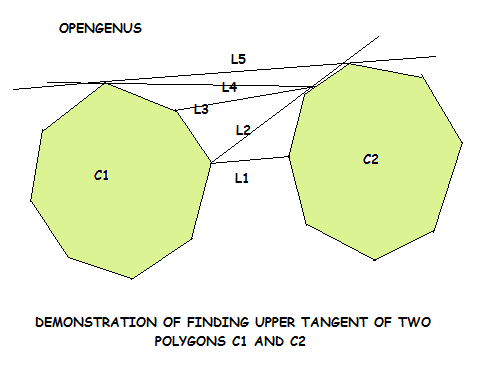
\includegraphics[scale=0.6]{convex_tangent}\\
Otrzymujemy algorytm:
\begin{python}
L = wewnetrzne(C1,C2)
while flag:
    flag = False
    while przecina(L, C1):
        przesun_wyzej(L, C1)
    while przecina(L, C2):
        flag = True
        przesun_wyzej(L, C2)
\end{python}
Funkcję $przecina(L,C)$ możemy zaimplementować korzystając z iloczynu wektorowego, dokładnie jego znaku, który określa nam skrętność, używając punktów określających $L$ w obu otoczkach i ich następników.\\\\
$przesun\_wyzej$ przesuwa punkt wyżej w danej otoczce: $v = C[(idx+1)\%n]$\\
Analogicznie znajdujemy odcinek na dole otoczek.\\
\subsection*{Poprawność}
Otrzymujemy wielokąt wypukły, odcinki łączące $C_1, C_2$ nie przecinają ich (dopiero wtedy kończymy pętlę).\\
$C_1, C_2$ zawierają wszystkie punkty, więc zbiór w którym obie się one zawierają też zawiera wszystkie punkty.\\
\clearpage
\subsection*{zadanie 4a}
Na początku zmodyfikujmy (liniowo) nasze drzewo tak aby każdy wierzchołek $v$ miał $deg(v) \leq 3$. Zrobimy to dodając czarne wierzchołki (czerwone = oryginalne z drzewa) z zerowymi krawędziami w następujący sposób:\\
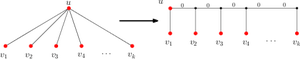
\includegraphics[scale=1.2]{czarne}\\
każdego nadmiarowego syna podpinamy do nowego czarnego którego łączymy z poprzednim czarnym wierzchołkiem.\\
Zerowe krawędzie gwarantują nam, że w tak zmodyfikowanym drzewie rozwiązanie się nie zmieni.\\\\
Korzystamy z metody \textit{Dziel i Zwyciężaj} dla danego wierzchołka $u$ i jego conajwyżej trzech poddrzew $T_1,T_2,T_3$ o korzeniach (sąsiadach $u$) $r_1,r_2,r_3$, odpowiedź to ścieżki wewnątrz każdego z poddrzew $T_i$, ścieżki pomiędzy poddrzewami $T_i, T_j$ (i ścieżki pomiędzy $T_i$ a $u$).\\
Dla danych $i,j$ ($i<j$) oznaczmy przez $w = d(u,r_i) + d(u,r_j)$, $A = v, v \in {T_i}$, $B = w, w \in T_j$. W $A,B$ trzymamy tylko czerwone wierzchołki.\\$A,B$ sortujemy po odległościach wierzchołków od korzeni np. $A$ po $d(v,r_i)$.\\\\
Teraz szukamy takich par $x,y, x\in A, y \in B$, że $d(x,r_i) + d(y,r_j) = D - w$\\
Możemy to zrobić w czasie liniowym (po wcześniejszym sortowaniu $A,B$) idąc od lewej w $A$ i od prawej w $B$.\\
Oszacujmy, złożoność takiego algorytmu:
$$
T(n) = \mathcal{O}(n\log{n}) + T(n_1) + T(n_3) + T(n_3)
$$
Aby złożoność nam nie wybuchła musimy jeszcze zadbać o to by rozmiary drzew wywołania rekurencyjnych były ograniczone lepiej niż $n$. \\Bo wiemy, że $n_1 + n_2 + n_3 = n-1$ w przeciwnym przypadku być może wykonamy $n$ wywołań otrzymując złożoność $\mathcal{O}(n^2\log{n})$.\\
Możemy to osiągnąć biorąc jako wierzchołek do usunięcia $u$ centroid obecnego drzewa, wtedy $n_i \leq \frac{n}{2}$, centroid można wyszukać w czasie $\mathcal{O}(n)$.\\
Każde wywołanie zmniejsza nam drzewo conajmniej dwukrotnie, więc pełne drzewo będzie \\
\clearpage
\begin{python}
def getAns(l1, l2):
    sort(l1)

def solve(G):
    u = centroid(G)
    ans = 0
    red = []
    for r in G[u]:
        G2 = subtree(r)
        red.append(getRed(G2))
        ans += solve(G2)
    for (i,j) in list(combinations(range(3), 2)):
        ans += getAns(red[i],red[j])

dodaj_czarne(G)
\end{python}
\end{document}

